
%%%%%%%%
\begin{frame}{What did they do?}
    \begin{quote}
        Fifty-six of 96 tumor specimens showed altered p53 expression.  The patients with altered p53 expression survived for a significantly shorter period after surgery than those without p53 expression, (P = 0.02, [...] Wilcoxon test). 
    \end{quote}
    \figcaption{Fujino et al 1995, \textit{Prognostic significance of p53 and ras p21 expression in nonsmall cell lung cancer}}

    \pause

    Recorded survival times for 56 patients with altered p53 expression and 40 patients without;
    did a Wilcoxon-Mann-Whitney test comparing the two groups.

\end{frame}

%%%%%%%%
\begin{frame}{What did they do?}

    \emph{DNA methylation profiling in breast cancer discordant identical twins identifies DOK7 as novel epigenetic biomarker}, Heyn et al 2013

    \vspace{1em}

    \begin{quote}
        DNA methylation level is [a property of sites in the genome, and is] displayed as beta-values ranging from 0--1. 
        To identify consistently differentially methylated CpG sites [in the genome] Wilcoxon rank sum paired test was performed for normalized beta-values of paired twins. 
    \end{quote}

\end{frame}

%%%%%%%%
\begin{frame}{}

    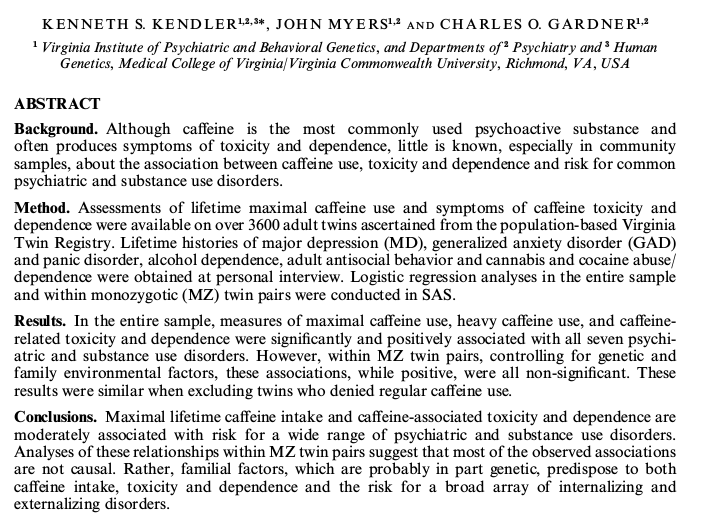
\includegraphics[width=\textwidth]{caffeine-twin-study}

\end{frame}


